\section{Microeconomics Midterm 21 / 22}

{
\subsection*{Schmidt}

{
\subsubsection*{Exercise 1}

\begin{enumerate}[label=(\alph*)]
{\item 
Clearly, WA is violated as $15 \in[0.22 .5]$ by the result in (b).
}
{\item 
WA: if $x \neq x^{\prime}$ and $p^{\prime} x \leqslant w^{\prime} \Rightarrow p x^{\prime}>w$

Thus check bundles in other price-wealth situations:

$$
\begin{aligned}
\left|\begin{array}{l}
4 \cdot 30+8 \cdot y=120+8 y \leqslant w_{0}=4 \cdot 15+8 \cdot 30=300 \\
12 \cdot 15+6 \cdot 30=360 \leqslant w_{1}=12 \cdot 30+6 y=360+6 y \\
\end{array}\right| \\
\Leftrightarrow\left|\begin{array}{l}
y \leqslant 22.5 \\
0 \leqslant y
\end{array}\right|
\Longleftrightarrow y \in[0.22 .5]
\end{aligned}
$$

$W A$ is violated if $y \in[0,22.5]$.
}
\end{enumerate}
}
{
\subsubsection*{Exercise 2}

\begin{enumerate}[label=(\alph*)]
{\item 
Use Roy's identity:

$$
x_{l}(p, w)=-\frac{\frac{\partial v(p, w)}{\partial p_{l}}}{\frac{\partial v(p, w)}{\partial w}}
$$

Then let $f(\cdot)$ be a movotonic tranformation:

$$
\tilde{x}_{l}(p, w)=-\frac{\frac{\partial f(v(p, w))}{\partial p_{l}}}{\frac{\partial f(p, w))}{\partial w}}=-\frac{\frac{\partial f(p, w)}{\partial v(p, w)}}{\frac{\partial f(p, w)}{\partial v(p, w)}} \frac{\frac{\partial v(p, w)}{\partial p_{l}}}{\frac{\partial v(p, w)}{\partial w}}=x_{l}(p, w)
$$
}
{\item 
(1) find $w(v(p, w))$ :

$$
w=\left(\frac{p_{1}}{\alpha}\right)^{\alpha}\left(\frac{p_{2}}{1-\alpha}\right)^{1-\alpha} v(p, w)
$$

At optimum: $w=e(p, u)$ and $v(p, w)=u$.

(2) Apply Shephard's Lemma to e(p,u):

$$
\begin{aligned}
h_{1}(p, u)=\frac{\partial e\left(p_{1} u\right)}{\partial p_{1}} & =\alpha\left(\frac{1}{\alpha}\right)^{\alpha}\left(\frac{p_{2}}{p_{1}(1-\alpha)}\right)^{1-\alpha} u \\
& =\left(\frac{p_{2}}{p_{1}} \frac{\alpha}{1-\alpha}\right)^{1-\alpha} u
\end{aligned}
$$
}
{\item 
case 1:

$$
\begin{aligned}
& \alpha=\alpha\left(p_1 / p_{2}\right) \longrightarrow \alpha\left(\lambda p_{1} / \lambda p_{2}\right)=\alpha \\
& h_{1}\left(\lambda p_{1}, u\right)=\left(\frac{\lambda p_{2}}{\lambda p_{1}} \frac{\alpha}{1-\alpha}\right)^{1-\alpha} u \\
& =\left(\frac{p_{2}}{p_{1}} \frac{\alpha}{1-\alpha}\right)^{1-\alpha} u=h_{1} (p_{1}, u)
\end{aligned}
$$

case 2: $\alpha=\alpha\left(p_{1}\right)$

$$
\begin{aligned}
h_{1}(\lambda p_1, u) & =\left(\frac{\lambda p_{2}}{\lambda p_{1}} \frac{\alpha\left(\lambda {p_{1}}\right)}{1-\alpha \left(\lambda p_{1}\right)}\right)^{1-\alpha\left(\lambda_{p_{1}}\right)} u \\
& =\left(\frac{p_{2}}{p_{1}} \frac{\alpha\left(\lambda p_{1}\right)}{1-\alpha\left(\lambda {p_{1}}\right)}\right)^{1-\alpha\left(\lambda_{p_{1}}\right)} u \neq h_{1}\left(p_{1} , u\right)
\end{aligned}
$$
}
\end{enumerate}
}
{
\subsubsection*{Exercise 3}

The difference between consumer theory and production theory is mainly the fact that firms do not have budget constraints.
This problem introduces a budget constraint. Therefore, we are going to treat the problem like a consumer problem.
In that sense, the revenue is comparable to the utility function, and the cash constraint is like the wealth of a consumer.
Consequently, we are solving the following revenue maximization problem (which is the analogue to a utility maximization problem):

\begin{align*}
    \max_{z_1,z_2} pf(z_1,z_2) \\
    \operatorname{s.t.} \; w_1z_1 + w_2z_2 \leq C
\end{align*}

We will assume an interior solution (the budget constraint is binding).
Then, the revenue function $R(p, w_1, w_2, C)$ that the exercise gives us is just the equivalent to the indirect utility.

\begin{enumerate}[label=(\alph*)]
{\item 
As $R(p, w_1, w_2, C)$ works like the indirect utility, we apply Roy's identity to find the factor demand, which is the analogue to the Walrasian demand:

\begin{align*}
    z_1&=-\frac{\frac{\partial R}{\partial w_1}}{\frac{\partial R}{\partial C}} \\
    &= -\frac{p \cdot(-\alpha) \frac{1}{w_1}}{p \cdot \frac{1}{C}} \\
    &= \alpha \frac{C}{w_1}
\end{align*}
}
{\item 
We treat $R(p,w,C)$ as the indirect utility depending on income and invert it to find the cost function $C(p,w,R)$, which is the analogue to the expenditure function in consumer theory:

\begin{align*}
    R&=p\left[\gamma+\ln C(p,w,R)-\alpha \ln w_1-(1-\alpha) \ln w_2\right] \\
    \frac{R}{p}-\gamma &= \ln \left(\frac{C(p,w,R)}{w_1^\alpha w_2^{1-\alpha}} \right) \\
    \exp\left(\frac{R}{p}-\gamma\right)&=\frac{C(p,w,R)}{w_1^\alpha w_2^{1-\alpha}} \\
    C(p,w,R) &= w_1^\alpha w_2^{1-\alpha}\exp\left(\frac{R}{p}-\gamma\right)
\end{align*}
}
{\item 
Since the cost function from (b) happens to be the analogue to the expenditure function, we can apply Shephard's Lemma in order to find the factor demand for a given $R$ at minimum cost, as this is the analogue to the Hicksian demand in consumer theory.
In that spirit, let us call this function $h_1(p,w,R)$.

\begin{align*}
    h_1(p,w,R)&=\frac{\partial C\left(w,R\right)}{\partial w_1} \\
    &= \alpha \exp \left[\frac{R}{p}-\gamma\right] \cdot\left(\frac{w_2}{w_1}\right)^{1-\alpha}
\end{align*}
}
{\item 
In consumer theory, the Hicksian demand and the Walrasian demand meet at optimum. We can also show that here:

\begin{align*}
    h_1(w,R)&=z_1^* \\
    \alpha \exp \left[\frac{R}{p}-\gamma\right] \cdot\left(\frac{w_2}{w_1}\right)^{1-\alpha}&=\alpha \frac{C}{w_1}\\
    \exp \left[\frac{R}{p}-\gamma\right] w_1^\alpha w_2^{1-\alpha}&=C \\
    \frac{R}{p}-\gamma &= \ln \left(\frac{C}{w_1^\alpha w_2^{1-\alpha}} \right) \\
    R&=p\left[\gamma+\ln C-\alpha \ln w_1-(1-\alpha) \ln w_2\right]
\end{align*}

The last line is exactly the formula for the revenue that is observed by our econometrician friend in the optimum. Therefore, we have shown that the two demands are equal whenever the firm is acting optimally, i.e. maximizing its revenue or minimizing its cost. Put differently, the revenue maximization problem is the dual problem to the cost minimization problem and vice versa.
}
\end{enumerate}
}
{
\subsubsection*{Exercise 4}

\begin{enumerate}[label=(\alph*)]
{\item 
\underline{IF:}

$u(x)=\beta x^{1-\rho}+\gamma$

$$
r^{R}=-x \frac{u^{\prime \prime}(x)}{u^{\prime}(x)}=-x \frac{\beta(1-  \rho)(-\rho) x^{-\rho-1}}{\beta(1-\rho) x^{-\rho}}=\rho
$$

\underline{ONLY IF:}

$r^{R}=-x \frac{u^{\prime \prime}(x)}{u^{\prime}(x)}=-x \frac{\partial \ln \left(u^{\prime}(x)\right)}{\partial x}=\rho$

$$
\begin{aligned}
& \Longleftrightarrow \quad \frac{\partial \ln \left(u^{\prime}(x)\right)}{\partial x}=-\rho \frac{1}{x} \\
& \Longleftrightarrow \int_{\underline{x}}^{x} \frac{\partial \ln \left(u^{\prime}(t)\right)}{\partial t} d t=-\rho \int_{\underline{x}}^{x} \frac{1}{t} d t \\
& \Longleftrightarrow \quad \ln \left(u^{\prime}(x)\right)-\ln \left(u^{\prime}(\underline{x})\right)=-\rho (\ln (x)-\ln (\underline{x})) \\
& \Leftrightarrow \quad u^{\prime}(x)=x^{-p} \frac{u^{\prime}(\underline{x})}{\underline{x}^{-\rho}}=x^{-\rho} \alpha \\
& \int_{\underline{x}}^{x} u^{\prime}(y) d y=\alpha \int_{\underline{x}}^{x} y^{-\rho} d y \\
& \Leftrightarrow \quad u(x)-u(\underline{x})=\frac{\alpha}{1-\rho}\left(x^{1-p}-\underline{x}^{1-p}\right) \\
& \Leftrightarrow \quad u(x)=\beta x^{1-p} + \gamma
\end{aligned}
$$

Risk aversion:

$$
\begin{aligned}
& u^{\prime \prime}(x)<0 \\
\Leftrightarrow &\beta(1-\rho)(-\rho) x^{-\rho-1}<0 \\
\Rightarrow &\beta(1-\rho) {\rho}>0
\end{aligned}
$$

This only holds when $(\beta>0$ and $\rho<1)$ or $(\beta<0$ and $\rho>1$ ).
}
\end{enumerate}
}
}

\newpage
{
\subsection*{Gottardi}

{
\subsubsection*{Exercise 1}

\begin{enumerate}[label=(\roman*)]
{\item 
Pareto Efficient:

\begin{align*}
    M R S^{A}=3 \frac{x_{2}^{A}}{x_{1}^{A}}&=M R S^{B}=\frac{1}{2} \\
    \Longleftrightarrow \quad x_{2}^{A}&=\frac{1}{6} x_{1}^{A}
\end{align*}

\begin{figure}[!htp]
    \centering
    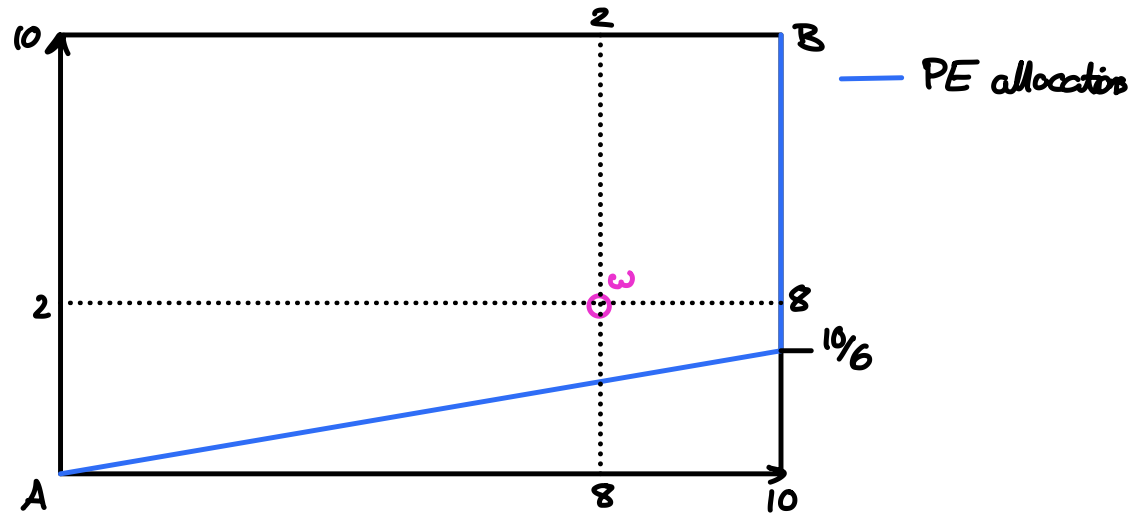
\includegraphics[width=.75\textwidth]{images/2021_22_1.png}
\end{figure}
}
{
\item 
\underline{consumer A:}

$$
\begin{aligned}
& \max _{x_{1}^{A}, x_{2}^{A}} 3 \ln \left(x_{1}^{A}\right)+\ln \left(x_{2}^{A}\right) \\
& \text { s.t. } x_{1}^{A}+p x_{2}^{A}=8+2 p 
\end{aligned}
$$

FOCs:

$$
\begin{aligned}
& \left[x_{1}^{A}\right]: \frac{3}{x_{1}^{A}}-\lambda=0 \\
& \left[x_{2}^{A}\right]: \frac{1}{x_{2}^{A}}-\lambda p=0 \\
& \rightarrow x_{1}^{A}=3 p x_{2}^{A}
\end{aligned}
$$

\underline{consumer B:} linear utility leads to:

$$
\begin{aligned}
& x_{1}^{B}=\left\{\begin{array}{lll}
\infty & \text { if } & p \geq 2 \\
\mathbb{R}^{+} & \text { if } & p=2 \\
0 & \text { if } & p<2
\end{array}\right. \\
& x_{2}^{B}=\left\{\begin{array}{lll}
\infty & \text { if } p \leq 2 \\
\mathbb{R}^{+} & \text { if } p=2 \\
0 & \text { if } p>2
\end{array}\right.
\end{aligned}
$$

\underline{market:} 

$$
x_{1}^{A}+x_{1}^{B}=10=x_{2}^{A}+x_{2}^{B}
$$

In order for markets to clear with no excess demand, we must have $p=2$ because of consumer B's preferences.
Therefore

$$
x_{1}^{A}=6 x_{2}^{A}
$$

plug into $B C^{A}: \quad 8 x_{2}^{A}=8+4 \quad \Longleftrightarrow x_{2}^{A}=12 / 8=3 / 2$

$$
\rightarrow x_{1}^{A}=9 \rightarrow\left(x_{1}^{B}, x_{2}^{B}\right)=(1,17 / 2)
$$

\underline{Competitive Equilibrium:}

\begin{align*}
    \left(x_{1}^{A}, x_{2}^{A}\right) &= (9,3 / 2) \\
    \left(x_{1}^{B}, x_{2}^{B}\right) &= (1,17 / 2) \\
    \frac{p_2}{p_1} &= 2
\end{align*}

Since $x_{2}^{A}=1 / 6 x_{1}^{A}$, PE is achieved.
}
{
\item 

$$
\begin{aligned}
& u^{A}\left(w_{1}^{A}, w_{2}^{A}\right)=3 \ln (8)+\ln (2) \cong 6.931 \\
& u^{A}\left(x_{1}^{A}, x_{2}^{A}\right)=3 \ln (9)+\ln (3 / 2) \cong 6.997 \\
& u^{B}\left(w_{1}^{B}, w_{2}^{B}\right)=2+2 \cdot 8=18 \\
& u^{B}\left(x_{1}^{D}, x_{2}^{B}\right)=1+2 \cdot 17 / 2=18
\end{aligned}
$$

By FWT this is always true, when preferences do not violate LNS, there is free disposal and markets are complete.
}
\end{enumerate}
}
{
\subsubsection*{Exercise 2}

Autarky: A sells, B buys good 1.

Effect depends on price change \& preferences.

Assume $\frac{P_1}{P_2}$ goes up (the other way round the argument can be reversed).
This makes the seller better off as she gets more per unit sold and might even sell more. For $B$ it depends on her preferences. If she can substitute and switch to selling good 1, she profits. 
If she has to buy good 1 at a higher price, she loses. It is also possible that her utility does not change despite the price change. 

If prices remain the same, nothing changes.
}
{
\subsubsection*{Exercise 3}

$$
\left(w_{1}, w_{2}\right)=(1,4)
$$

\begin{enumerate}[label=(\roman*)]
{\item 
at $t=0: \quad q_{1} \theta_{1}+q_{2} \theta_{2}=0$

at $t=1, s=1: \quad x_{1}=w_{1}+\theta_{1} 4+\theta_{2}$

at $t=1, s=2: \quad x_{2}=w_{2}+\theta_{2}$
}
{
\item 

\underline{Consumer problem:}

$$
\begin{gathered}
\max _{\theta_{1}, \theta_{2}} 1 / 4\left(w_{1}+4 \theta_{1}+\theta_{2}\right)^{1 / 2}+3 / 4\left(w_{2}+\theta_{2}\right)^{1 / 2} \\
\text { s.t. } \quad q_{1} \theta_{1}+q_{2} \theta_{2}=0
\end{gathered}
$$

FOCs:

\begin{align*}
    &\left[\theta_{1} \right]: \frac{4}{8\left(w_{1}+4 \theta_{1}+\theta_{2}\right)^{1 / 2}}-\lambda q_{1}=0 \\
    &\left[\theta_{1} \right]: \frac{1}{8\left(w_{1}+4 \theta_{1}+\theta_{2}\right)^{1 / 2}}+\frac{3}{8\left(w_{2}+\theta_{2}\right)^{1 / 2}}-\lambda q_{2}=0
\end{align*}

\underline{market clearing:}

\begin{align*}
    \theta_{1}=-\theta_{2}=0 \tag{I}
\end{align*}

Plug (I) into FOCs:

$$
\begin{aligned}
& \frac{1}{2}=\lambda q_{1} ; \quad \frac{1}{8}+\frac{3}{16}=\lambda q_{2} \\
\longrightarrow & \frac{q_{1}}{q_{2}}=\frac{1}{2} \frac{16}{5}=\frac{8}{5}
\end{aligned}
$$
}
{
\item 

$\mathbb{E}\left(r_{1}\right)=\mathbb{E}\left(r_{2}\right)=1$

$$
\longrightarrow \frac{\mathbb{E}\left(r_{1}\right)}{q_{1}}>\frac{\mathbb{E}\left(r_{2}\right)}{q_{2}} \Longleftrightarrow 1>\frac{q_{1}}{q_{2}}=\frac{8}{5}
$$

We see that the inequality above is INCORRECT, we have run into a CONTRADICTION.

Usual intuition: $q_{1} / q_{2}>1$ because consumer wants to insure against poor state where she has less income. This leads to a lower expected rate of return for asset 1. Otherwise the consumer would buy asset 1 but she cannot because of market clearing.
}
\end{enumerate}
}
}